% 保留原始面板、实拍、示例与全部连线；仅以 TikZ 覆盖说明标签。
\begin{tikzpicture}
\node[anchor=south west,inner sep=0] (im) at (0,0) {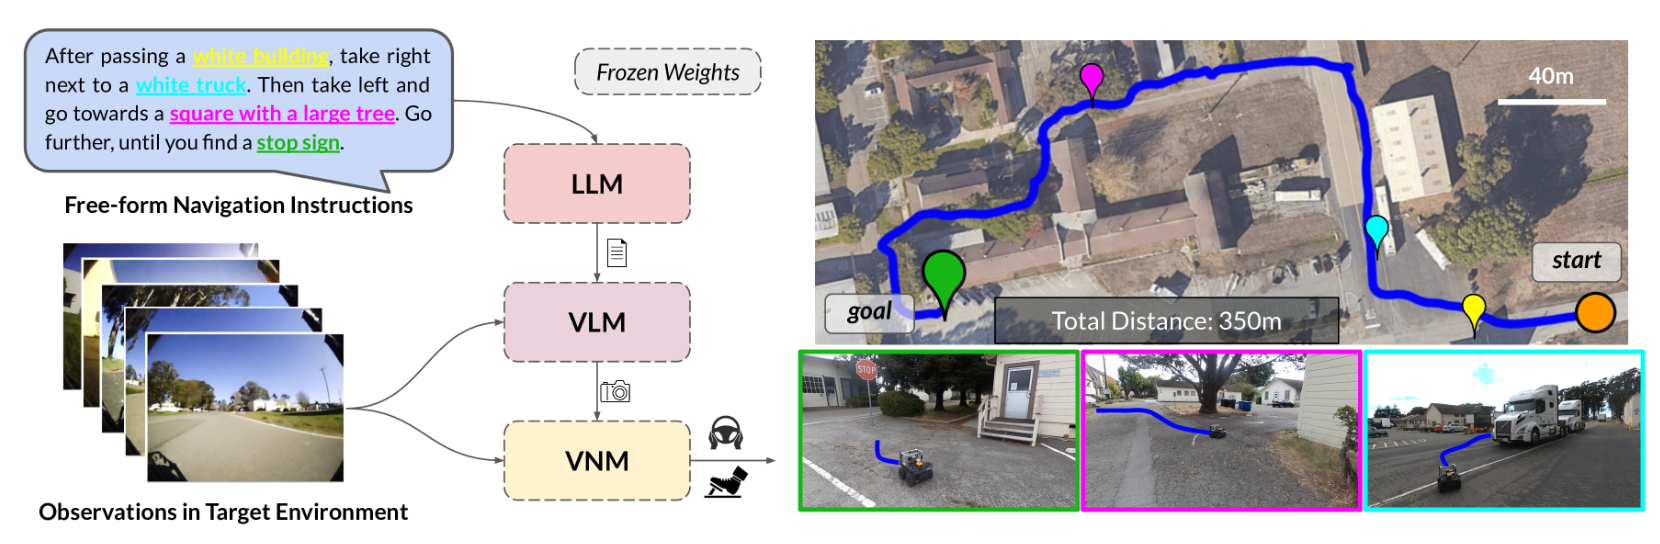
\includegraphics[width=\linewidth]{figures/lmnav.png}};
\begin{scope}[x={(im.south east)},y={(im.north west)}]
\fill[blue!12] (0.022892,0.698529) rectangle (0.266265,0.943015);
\node[align=center,inner sep=0pt,font=\fontsize{7.2}{8.2}\selectfont,text width=0.243373\linewidth,rotate=0] at (0.144578,0.820772) {经过白色建筑后，在白色卡车旁右转。然后左转，前往有大树的广场。继续走，直到找到停止标志。};
\fill[white] (0.031325,0.593750) rectangle (0.259036,0.648897);
\node[align=center,inner sep=0pt,font=\fontsize{8.5}{9.5}\selectfont,text width=0.227711\linewidth,rotate=0] at (0.145181,0.621324) {自由形式导航指令};
\fill[white] (0.351807,0.840074) rectangle (0.454217,0.904412);
\node[align=center,inner sep=0pt,font=\fontsize{8}{9}\selectfont,text width=0.102410\linewidth,rotate=0] at (0.403012,0.872243) {冻结权重};
\fill[white] (0.017470,0.022059) rectangle (0.266265,0.082721);
\node[align=center,inner sep=0pt,font=\fontsize{8.5}{9.5}\selectfont,text width=0.248795\linewidth,rotate=0] at (0.141867,0.052390) {目标环境中的观测};
\fill[gray!30] (0.602410,0.380515) rectangle (0.802410,0.448529);
\node[align=center,inner sep=0pt,font=\fontsize{8.5}{9.5}\selectfont,text width=0.200000\linewidth,rotate=0] at (0.702410,0.414522) {总距离：350 米};
\fill[gray!15] (0.928313,0.487132) rectangle (0.973494,0.544118);
\node[align=center,inner sep=0pt,font=\fontsize{8}{9}\selectfont,text width=0.045181\linewidth,rotate=0] at (0.950904,0.515625) {起点};
\fill[gray!15] (0.500000,0.391544) rectangle (0.542169,0.452206);
\node[align=center,inner sep=0pt,font=\fontsize{8}{9}\selectfont,text width=0.042169\linewidth,rotate=0] at (0.521084,0.421875) {终点};
\end{scope}
\end{tikzpicture}
